\section*{Задание}
В одной программе написать правила, позволяющие найти:
\begin{enumerate}
	\item Максимум из двух чисел
	\begin{enumerate}
		\item без использования отсечения;
		\item с использованием отсечения.
	\end{enumerate}
	\item Максимум из трех чисел
	\begin{enumerate}
		\item без использования отсечения;
		\item с использованием отсечения.
	\end{enumerate}
\end{enumerate}

\begin{lstinputlisting}[label=third,caption=Решение задания №1, language=prolog, firstline=1, lastline=47]{../src/lab_15.pro}
\end{lstinputlisting}

\begin{figure}[H]
	\caption{Таблица к заданию.}
	\begin{center}
		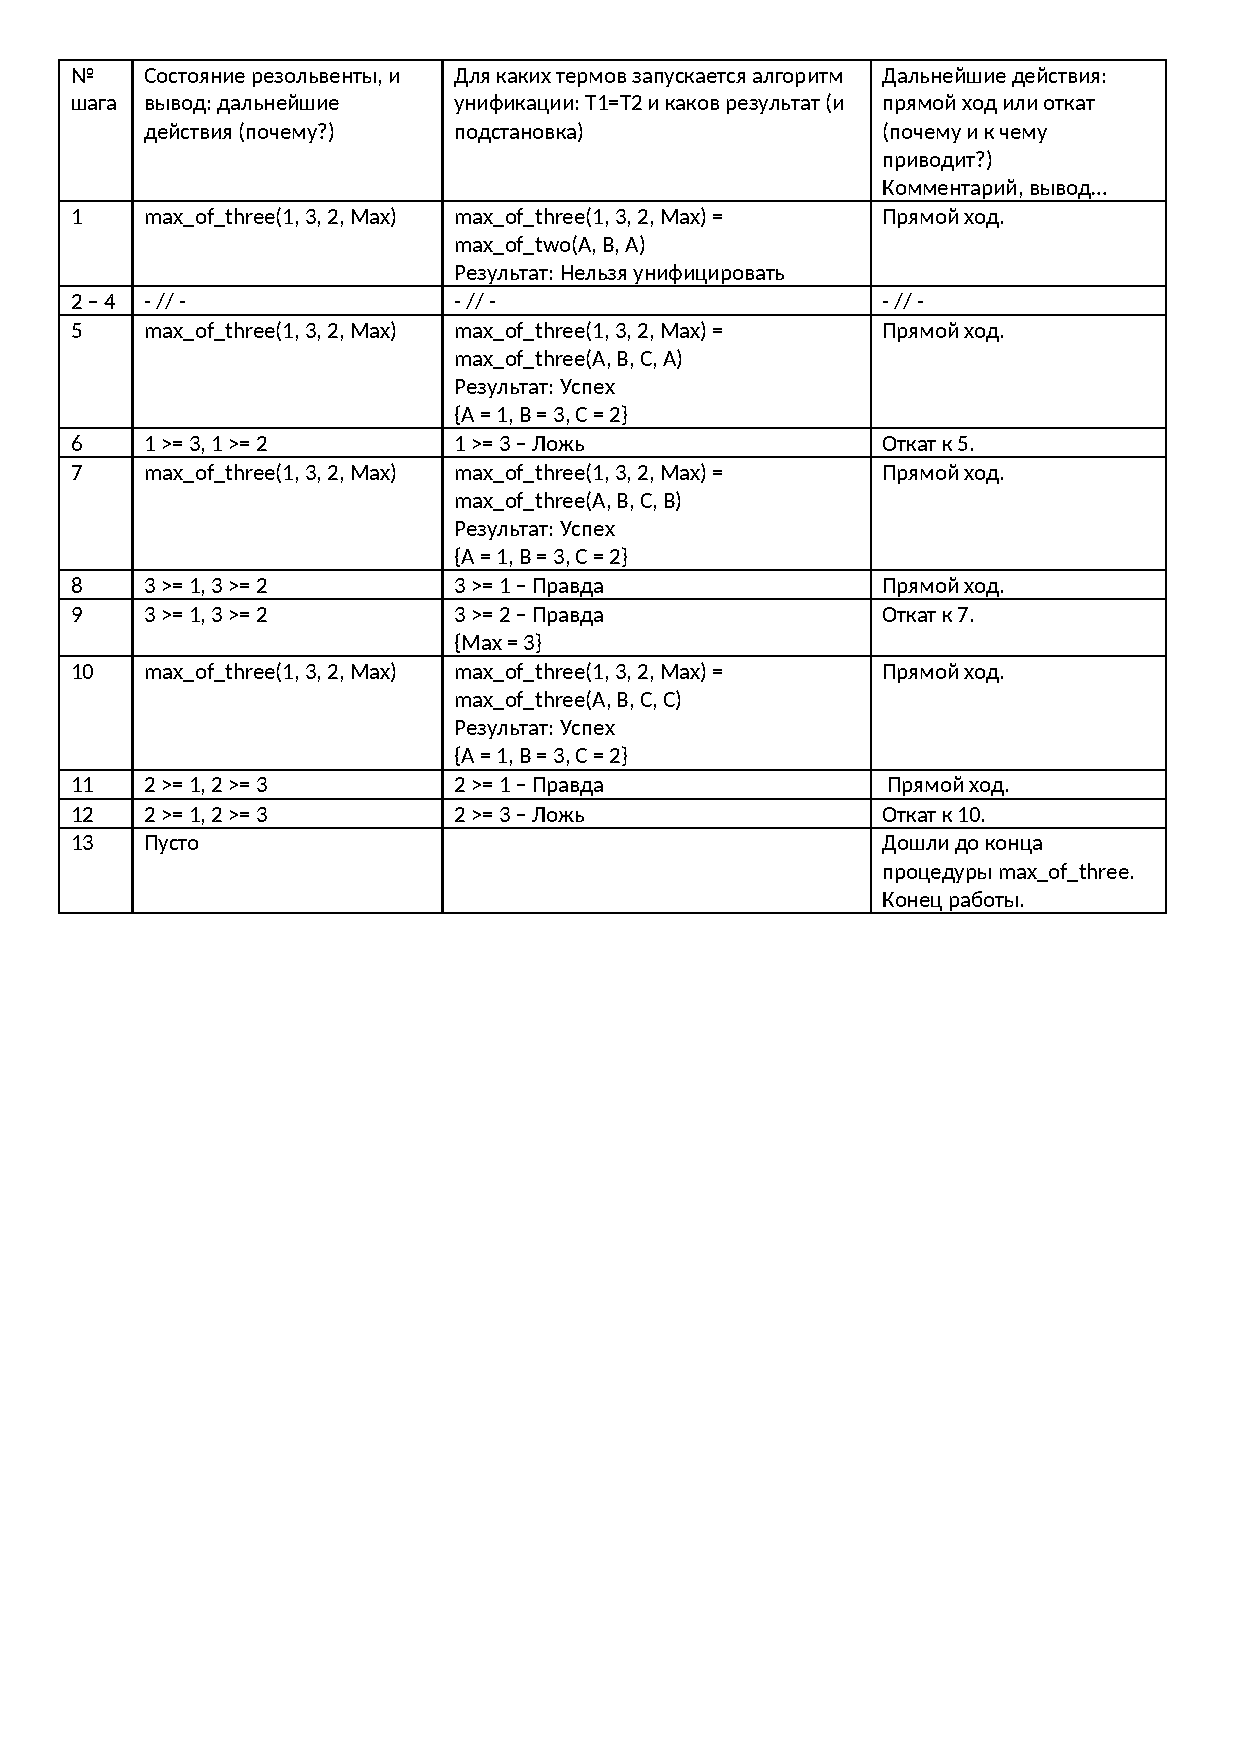
\includegraphics[scale=0.85]{img/15.1.pdf}
	\end{center}
	
\end{figure}

\begin{figure}[H]
	\begin{center}
		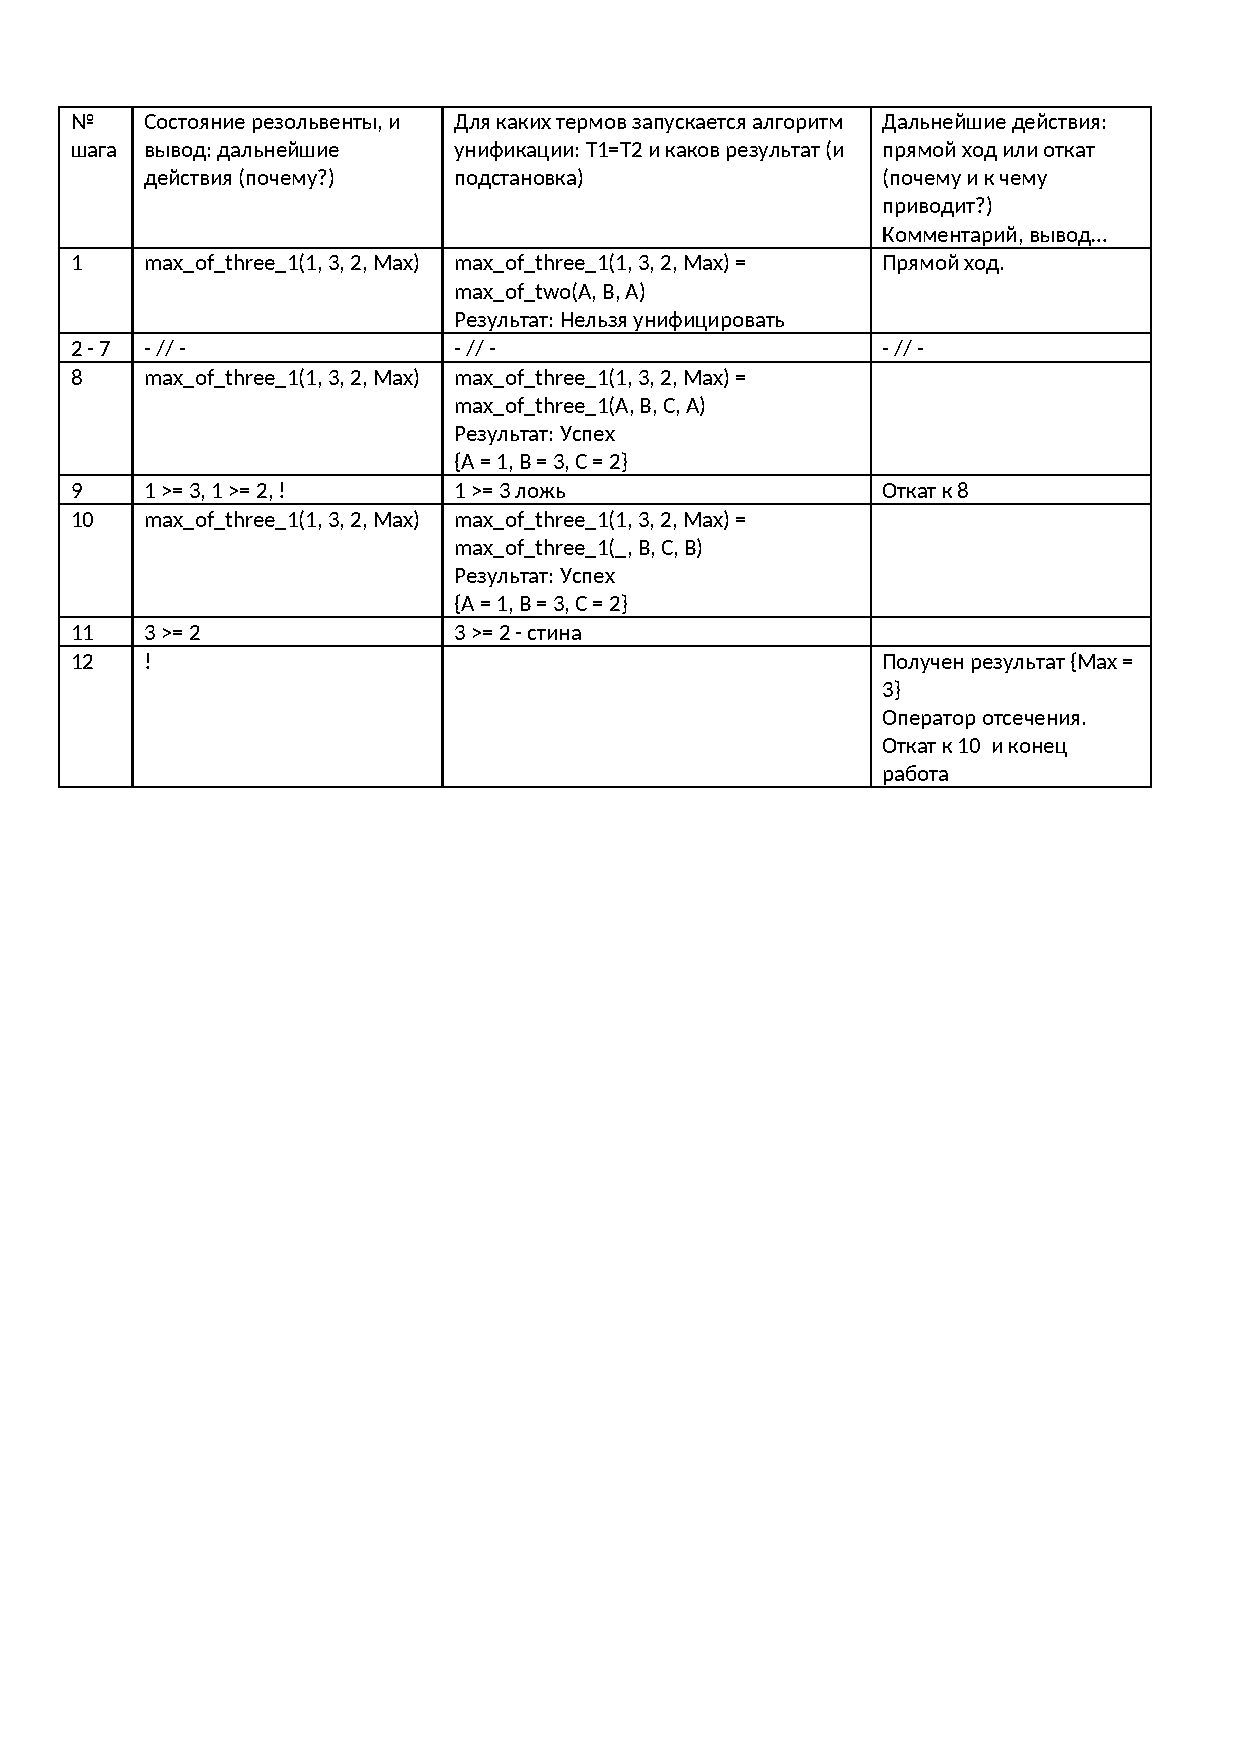
\includegraphics[scale=0.85]{img/15.2.pdf}
	\end{center}
	
\end{figure}